\subsection{Bot Behavior}

There are several bots operating on the contents of the Wikipedia.
Many bots are sanctioned by the community, and do useful
chores such as automatically removing text which is likely
to be vandalism, correcting spelling, and adding geographical data.
There are also bots which are created to vandalize pages,
and sometimes well-intentioned bots run amock and
accidentally vandalize pages as well.
During the course of comparing the various contribution
measures with each other, we found several bots (both
good and bad) which were obvious outliers in the data.
To analyze bots as a group, we selected all users
which included the ``Bot'' moniker in their username;
this self-identification does include some malicious bots,
but obviously favors selection of good bots.

The edit and text quality measures for all bots are similar to
that of all authors shown in Figure~\ref{fig-revs-quality}.
We noticed that bots create a large number of revisions with
high quality.
We found that $69.56\%$ of the revisions made by
bots have a text quality measure of $\textquality > 0.95$.
The percentage of revisions made by bots with 
$\textquality \le 0.05$ was $9.2\%$.
We found that $66.92\%$ of the new text added by bots were with
$\textquality > 0.95$ and $14.14\%$ of the new text added by
bots were with $\textquality = 0$, which means they were 
immediately reverted.
Similarly, on the edit contributions of bots we found that
$54.42\%$ of the revisions with edits made by bots were of
high edit quality, with $\avgeditquality > 0.9$.
The number of revisions having $\avgeditquality < -0.9$ being
negligible; $1\%$ from our analysis.
When we counted all edit revisions that had a negative edit
quality we saw that $12.73\%$ of the revisions were judged to 
be of poor quality with $\avgeditquality < 0$.
We found that $93.3\%$ of the edit contributions made by bots
had positive edit quality and the remaining $6.4\%$ had
negative edit quality.
More interestingly, $65.20\%$ of the edit contributions made
by bots had $\avgeditquality > 0.9$, which means they were
not edited out in subsequent revisions and represent the
sheer amount of work done by bots that is of very high quality.
The contributions with $\avgeditquality < -0.9$ are $1.8\%$.
This indicates that a large part of the text additions made by bots 
and a large part of the edit contributions made by bots survive
indefinitely.

Furthermore, our analysis indicates that bots make large amounts of
edit contributions compared to text contributions; the ratio
of the size of edits $\editonly$ to the size of new text $\textonly$
for all bots is $11.61$.
Since the penalizing measure $\punish$ does not credit authors for
good edits but reduces their $\textlong$ contributions, by the 
amount of their bad edits as measured by $\editlong$, we notice that 
edits judged as being of poor quality overwhelm the smaller text 
contributions of bots in general, and $AntiVandalBot$ in particular, 
resulting in a small overall contribution.
We also note here that $SmackBot$ did much better on this
measure.
$SmackBot$ contributes more text than $AntiVandalBot$.
Most of its edits are of smaller size than $AntiVandalBot$.
Since they have similar quality measures, $AntiVandalBot$ ends
up with a lower score on $\punish$ when compared to $SmackBot$.

\begin{comment}
%
\begin{figure*}
    \begin{center}
    \fbox{
    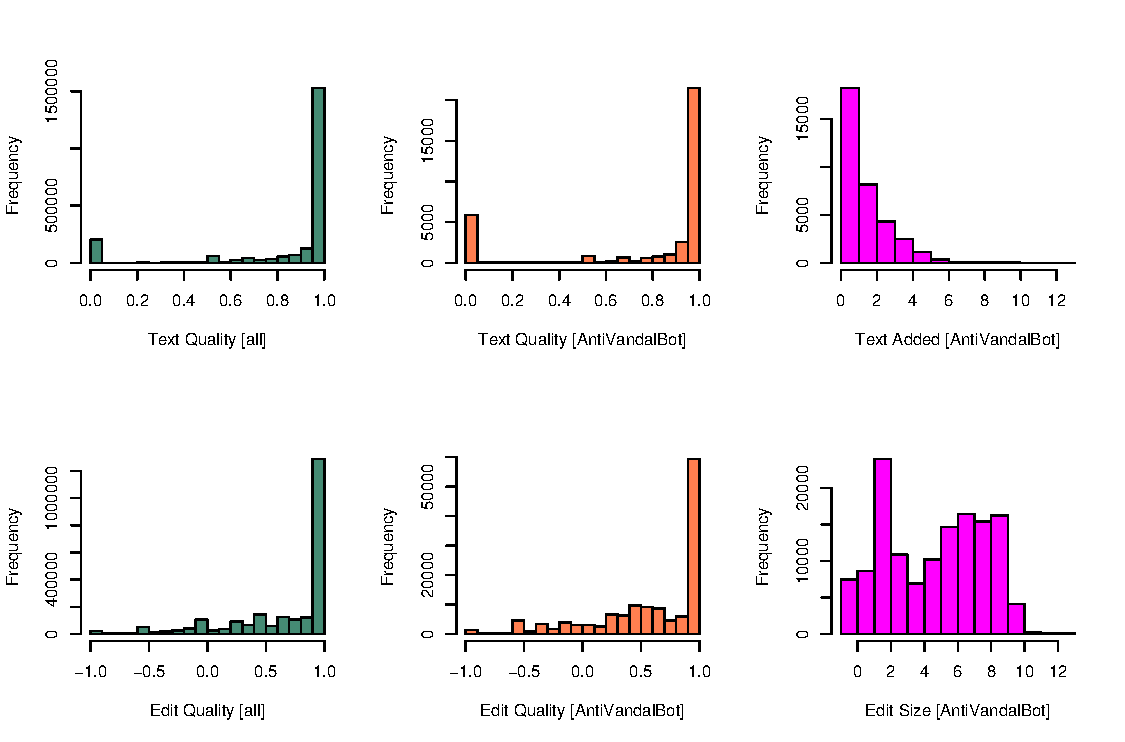
\includegraphics[scale=0.75]{part-I10-contrib/graphs/allbots_anti_hist}
    }
    \end{center}
    \caption[Measuring edit and text quality for all bots and $AntiVandalBot$]{
    	This graph shows the edit quality measure $\avgeditquality$
        and text quality $\textquality$ for all bots.
        A quality measure of $1$ indicates that all the changes
        were preserved.
        A quality measure of $0$ indicates that all the changes
        were reverted in the very next revision.
        The histograms on the left are for all bots.
        The ones on the right are the quality measures and the absolute amounts
        of text and edit contributions for $AntiVandalBot$.
    }
    \label{bot-contribs}
\end{figure*}
\end{comment}
